\documentclass[10pt]{beamer}

\usetheme{default}

\usepackage[utf8]{inputenc}
\usepackage[russian]{babel}
\usepackage[OT1]{fontenc}
\usepackage{amsmath}
\usepackage{amsfonts}
\usepackage{amssymb}
\usepackage{graphicx}
\usepackage{etoolbox}
\usepackage{caption}
\usepackage{subcaption}
\usepackage{pifont}

\makeatletter

\setbeamercolor{title}{fg=white}
\setbeamercolor{frametitle}{fg=black}
\setbeamerfont*{title}{family=\sffamily,size=\LARGE}

\setbeamerfont{page number in head/foot}{size=\scriptsize}
\setbeamertemplate{footline}[frame number]
\let\otp\titlepage
\renewcommand{\titlepage}{\otp\addtocounter{framenumber}{-1}}

\setbeamertemplate{background canvas}{%
	\ifnumequal{\c@framenumber}{0}{%
      
\includegraphics[width=\paperwidth,height=\paperheight]{images/cover.png}
   }{%
      \ifnumequal{\c@framenumber}{\inserttotalframenumber}{
         
\includegraphics[width=\paperwidth,height=\paperheight]{images/back.png}
      }{%
         % Other frames
      }%
   }%
}

\makeatother

\beamertemplatenavigationsymbolsempty

\author{Николай Анохин}
\title{\newline \newline \newline Лекция 1 \\ Задачи Data Mining}

\begin{document}

\begin{frame}[plain]
\titlepage
\end{frame}

\begin{frame}{Николай Анохин}

\begin{center}
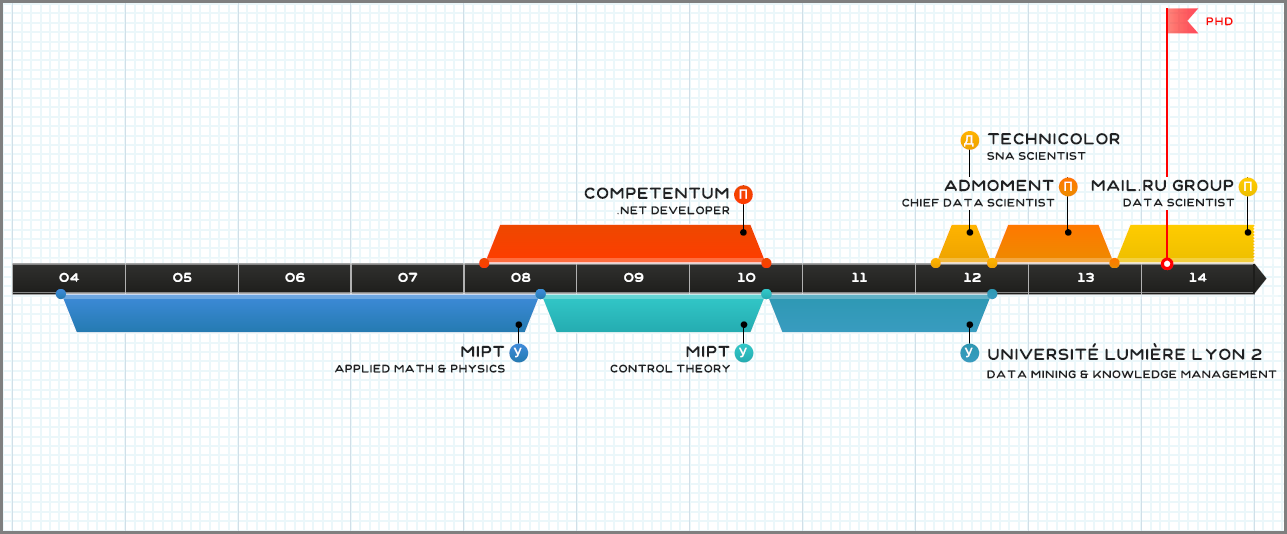
\includegraphics[scale=0.325]{images/timeline.png}
\end{center}

\begin{footnotesize}
e-mail: \href{mailto:n.anokhin@corp.mail.ru}{n.anokhin@corp.mail.ru} \\
тел.: +7 (903) 111-44-60
\end{footnotesize}

\end{frame}

\begin{frame}{План лекции}
\tableofcontents
\end{frame}

% =======================
\section{Структура курса}
% =======================

\begin{frame}{Структура курса}

{\small
Модуль 1
\begin{enumerate}
\item \underline{Задачи Data Mining (Николай Анохин)}
\item Задача кластеризации и EM-алгоритм (Николай Анохин)
\item Различные алгоритмы кластеризации (Николай Анохин){\color{red}$^{H}$}
\item Задача классификации (Николай Анохин)
\item Naive Bayes (Николай Анохин)
\item Линейные модели (Николай Анохин)
\item Метод опорных векторов (Николай Анохин){\color{red}$^{HP}$}
\end{enumerate}

Модуль 2
\begin{enumerate}
\item Снижение размерности пространства (Владимир Гулин)
\item Алгоритмические композиции 1 (Владимир Гулин)
\item Алгоритмические композиции 2 (Владимир Гулин){\color{red}$^{H}$}
\item Нейросети, обучение с учителем (Павел Нестеров){\color{red}$^{H}$}
\item Нейросети, обучение без учителя (Павел Нестеров)
\item Нейросети, глубокие сети (Павел Нестеров)
\end{enumerate}
}

\end{frame}

\begin{frame}{Контроль знаний}

\begin{block}{ДЗ}
4 домашних задания на 6-8 часов самостоятельной работы каждое (4x15 баллов)
\end{block}

\begin{alertblock}{Экзамен}
Презентация и защита семестрового проекта \\ (40 баллов)
\end{alertblock}

\end{frame}

\begin{frame}{Правила}

\begin{itemize}
\item[+] Можно задавать вопросы по ходу лекции
\item[+] Можно входить и выходить, не мешая коллегам
\item[---] Нельзя нарушать порядок в аудитории
\item[---] Нельзя разговаривать по телефону
\item Общение с преподавателем на ``Вы''
\end{itemize}

Ваши правила?

\end{frame}

% =======================
\section{Что такое Data Mining}
% =======================

\begin{frame}{DM как KDD}

\begin{block}{Data Mining}
Процесс извлечения знаний из различных источников данных, таких как базы данных, текст, картинки, видео и т.д. Полученные знания должны быть {\it достоверными}, {\it полезными} и {\it интерпретируемыми}.
\end{block}

\end{frame}

\begin{frame}{DM как моделирование}

\begin{block}{Data Mining}
Процесс построения модели, хорошо описывающей закономерности, которые порождают данные.
\end{block}

\vspace{1em}
Подходы к построению моделей
\begin{itemize}
\item[\color{green}\ding{52}] cтатистический
\item[\color{green}\ding{52}] на основании машинного обучения
\item[\color{red}\ding{54}] вычислительный
\end{itemize}

\end{frame}

\begin{frame}{DM и DS}

\begin{block}{Data Scientist}
Person who is better at statistics than any software engineer and better at software engineering than any statistician \\ (J. Wills, Data Scientist at Cloudera Inc.)
\end{block}

\vspace{1em}
Data-
\begin{itemize}
\item[\color{red}\ding{54}] -architecture
\item[\color{red}\ding{54}] -acquisition
\item[\color{green}\ding{52}] -analysis
\item[\color{red}\ding{54}] -archiving
\end{itemize}

\end{frame}

\begin{frame}{Success stories}

\begin{figure}
        \centering
        \begin{subfigure}[b]{0.45\textwidth}
                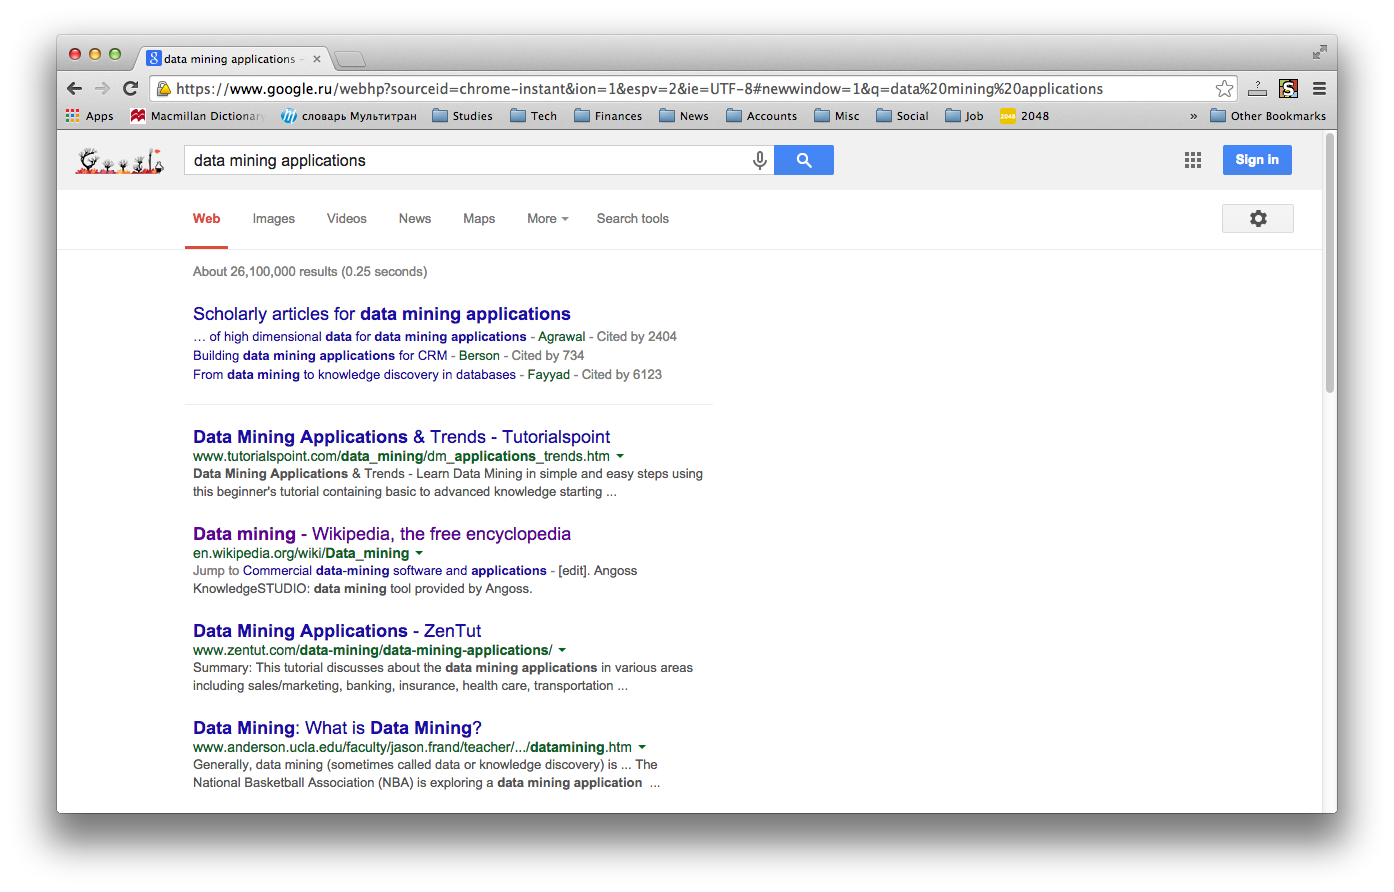
\includegraphics[width=\textwidth]{images/google.png}
                \caption{Google}                
        \end{subfigure}%        
        \begin{subfigure}[b]{0.45\textwidth}
                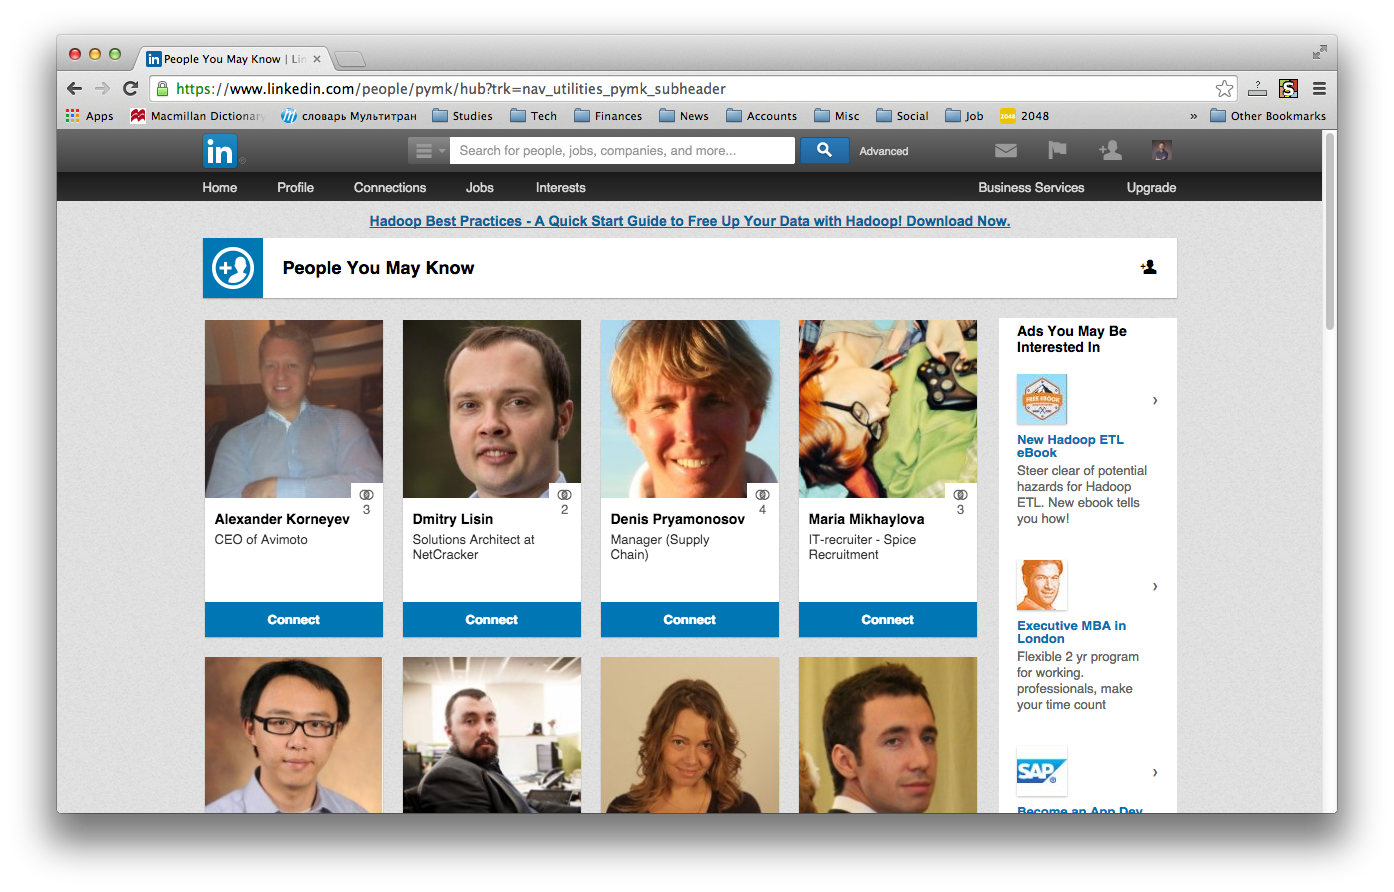
\includegraphics[width=\textwidth]{images/linkedin.png}
                \caption{LinkedIn}     
        \end{subfigure}
        
        \begin{subfigure}[b]{0.45\textwidth}
                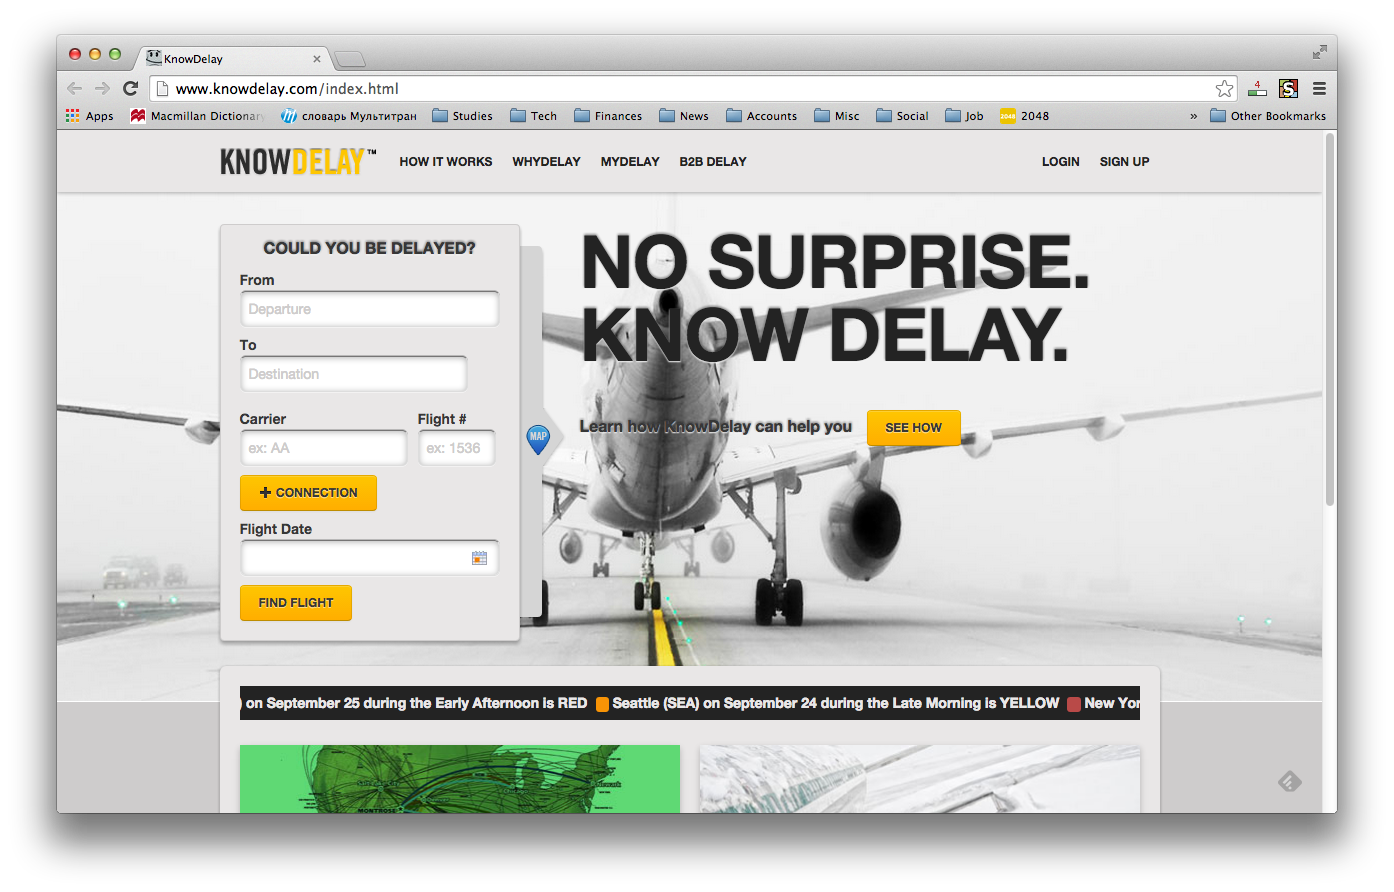
\includegraphics[width=\textwidth]{images/delay.png}
                \caption{KnowDelay}                
        \end{subfigure}%        
        \begin{subfigure}[b]{0.45\textwidth}
                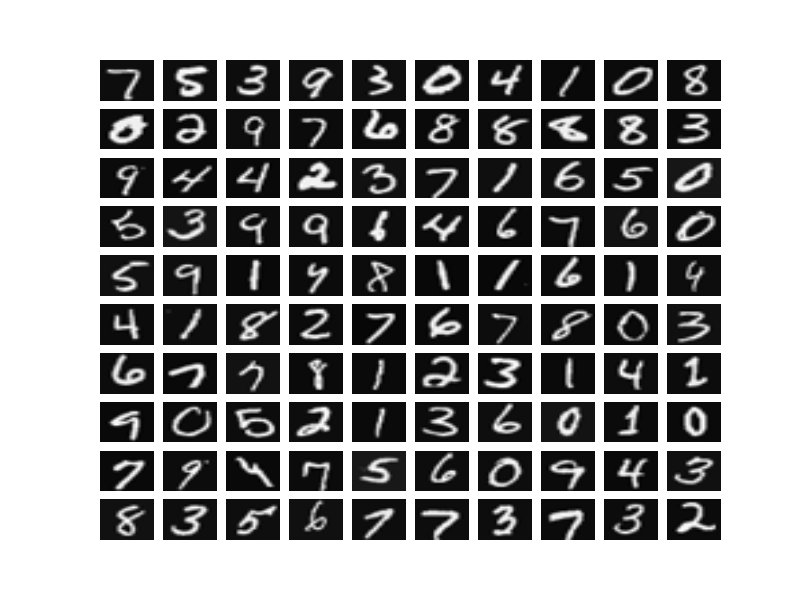
\includegraphics[width=0.9\textwidth]{images/digits.png}
                \caption{Handwritten digits}
        \end{subfigure}
\end{figure}

\end{frame}

\begin{frame}[plain]
\begin{center}
{\Large Вопросы}
\end{center}
\end{frame}

\end{document}